\documentclass[submitting]{nst}
\usepackage{subfigure,dcolumn}
\usepackage[T2A,T1]{fontenc}
\usepackage[english]{babel}

% The following package will be used to typeset the LaTeX codes and is not a necessity to this template
\usepackage{listings}
\lstloadlanguages{[LaTeX]TeX}
\lstset{language=[LaTeX]TeX,keywordstyle=\color{red},showspaces=true,breaklines=true,breakatwhitespace=true,basicstyle=\small\tt,commentstyle=\color{white},frame=single,framerule=0pt,backgroundcolor=\color{yellow}}


\begin{document}


\title{The MuTe simulation response to charged particles}

\author{A. Vásquez-Ramírez}
\email[Corresponding author:]{Carrera 27 calle 9 Ciudad Universitaria. Bucaramanga, Colombia., +57 3165084443, adrianacvr67@gmail.com}
\affiliation{Escuela de Física, Universidad Industrial de Santander, Bucaramanga Colombia}

\author{M. Suárez-Durán}
\affiliation{Departamento de F\'{\i}sica y Geolog\'{\i}a, Grupo de Investigación Integrar, Universidad de Pamplona, Pamplona-Colombia.}

\author{A. Jaimes-Motta}
\affiliation{Escuela de Física, Universidad Industrial de Santander, Bucaramanga Colombia}


\author{R. Calderón-Ardila}
\affiliation{Instituto de Tecnologías en Detección y Astropartículas, Centro Atómico Constituyentes,Comisión Nacional de Energía Atómica, Buenos Aires, Argentina}
\affiliation{Universidad Nacional de San Martín, Instituto SABATO, Argentina}

\author{J. Peña-Rodríguez}
\affiliation{Escuela de Física, Universidad Industrial de Santander, Bucaramanga Colombia}

\author{J.D. Sanabria-Gómez}
\affiliation{Escuela de Física, Universidad Industrial de Santander, Bucaramanga Colombia}

\author{D. Sierra-Porta}
\affiliation{Escuela de Física, Universidad Industrial de Santander, Bucaramanga Colombia}
\affiliation{Centro de Modelado Cient\'{\i}fico, Universidad del Zulia, 4001 Maracaibo-Venezuela}

\author{H. Asorey}
\affiliation{Instituto de Tecnologías en Detección y Astropartículas, Centro Atómico Constituyentes,Comisión Nacional de Energía Atómica, Buenos Aires, Argentina}
\affiliation{Laboratorio Detección de Partículas y Radiación,
Instituto Balseiro y Centro Atómico Bariloche,
Comisión Nacional de Energía Atómica, San Carlos de Bariloche, Argentina}
\affiliation{Sede Andina, Universidad Nacional de Río Negro, San Carlos de Bariloche, Argentina}


\author{L.A. Núñez}
\affiliation{Escuela de Física, Universidad Industrial de Santander, Bucaramanga Colombia}
\affiliation{ Departamento de Física, Universidad de Los Andes, Mérida, Venezuela}


\begin{abstract} 
abstract here
\end{abstract}

\keywords{keyword1, ... }

\maketitle
%%%%%%%%%%%%%%%%%%%
%%%% SECTION 1 %%%%
%%%%%%%%%%%%%%%%%%%
\section{Introduction}\label{sec:introduction}
The muography is an emerging technology based on measuring the attenuation of a muon flux that crosses geological and anthropic structures \cite{Kaiser2019}. Recently, we are witnessing several new successful academic and commercial applications such as detection of hidden materials in containers \cite{BlanpiedEtal2015}, archaeological building scanning \cite{MorishimaEtal2017, GomezEtal2016}, nuclear plant inspection \cite{FujiiEtal2013}, nuclear waste monitoring, underground cavities \cite{SaracinoEtal2017}, the overburden of railway tunnels \cite{ThompsonEtal2019} and volcanology (\cite{TanakaOlah2019} and references therein). In Colombia, more than a dozen active volcanoes, which represent significant risks to the nearby population \cite{Cortes2016, Agudelo2016, Munoz2017}, motivate research groups to explore this technique \cite{AsoreyEtal2017B, SierraPortaEtal2018, PenaRodriguezEtal2018, GuerreroEtal2019, ParraAvila2019}.  

Atmospheric muons originate from the decay of charged pions and kaons produced through the interaction of cosmic rays (\textsl{CRs}) with the nuclei of the Earth's upper atmosphere. The energy of these particles comprises a broad spectrum, but only those muons with the highest energies ($\sim 100$GeV) can cross hundreds of meters of rock \cite{MarteauEtal2012}. Besides, they are the most abundant charged particles that reach the sea level due to their high penetrating power (they only lose around $2$GeV when crossing the whole atmosphere) \cite{MarteauEtal2012}. Also, the muons are easily detectable concerning other particles, using different techniques based on ionization, excitation, and the Cerenkov effect \cite{MarteauEtal2012}. 

Hodoscopes are the most common detectors implemented for volcano muography.  They consist of two or several panels to identify the particle trajectories in terms of the zenith and azimuth angles. Projects like \textsl{MU-RAY} \cite{AnastasioEtal2013}, \textsl{ToMuVol} \cite{CarloganuEtal2013}, and \textsl{DIAPHANE} \cite{LesparreEtal2010} employ hodoscopes based on different detection technologies: emulsion plate, Resistive Plate Chambers, Micromegas, Multi-Wire Proportional Cameras, and scintillators, to mention the most common. Each of these techniques has advantages and disadvantages. The emulsion plate detectors \cite{MorishimaEtal2017, Nagamine2016} provide an excellent spatial resolution of the order of sub-microns, are passive, and easy to handle. On the other side, they have short lifetimes, and it is not possible to discriminate the time-stamp of dynamic phenomena, because the recorded events accumulate in the plates. The gas detectors as Resistive Plate Chambers \cite{SehgalEtal2016, Fehr2012}, Micromegas \cite{BouteilleEtal2016}, and Multi-Wire Proportional Cameras (\textsl{MWPCs}) \cite{OlahEtal2018}, allow obtaining short traces of the detected particles with a spatial resolution around the microns. However, since these detectors operate outdoors, the gain of the electrodes depends highly on environmental variables such as pressure and temperature. Besides, they require high voltage for optimal operation, which results in higher power consumption compared with emulsion detectors. Finally, there are scintillation detectors such as the segmented \cite{FujiiEtal2013, LesparreEtal2012, TanakaEtal2009} and continuous \cite{NagamineEtal1995, AguiarEtal2015, TangEtal2016},  that are more robust since these do not have a high mechanical variation with environmental conditions, are easily constructed at a much lower cost than gaseous and emulsion detectors. Nevertheless, their spatial resolution is not as good as the other detectors since the segments generally used are of the order of centimeters.

This paper presents the computational \textsl{Geant4} modeling of a hybrid Muon Telescope (\textsl{MuTe}) and the estimation of its response under a muon flux at $956$\,m a.s.l at Bucaramanga-Colombia. The model includes the materials, geometries, dimensions and the photo-sensitive devices of the detectors (see details in sections \ref{sec:hodoscope-response} and \ref{sec:wcd-response}). 

This paper presents the design, modeling and response of the \textsl{MuTe} detector, developed to perform the volcano muography technique in Colombia.


%%%%%%%%%%%%%%%%%%%
%%%% SECTION 2 %%%%
%%%%%%%%%%%%%%%%%%%

\section{The MuTe instrument design}
The Muon Telescope (sketched in figure \ref{fig:mute-detector}) is a hybrid detector that combines two technologies: a two-panel Scintillator Bars Hodoscope (\textsl{SBH}),  and a Water Cerenkov Detector (\textsl{WCD}), to filter most of the backward \& background noise \cite{NishiyamaMiyamotoNaganawa2014, KusagayaTanaka2015, NishiyamaEtal2016, GomezEtal2017}. This detector is capable of estimating not only the incoming  directions but also a range of energies of the impacting muons \cite{AsoreyEtal2017B}.
  
 The panels of the hodoscope consist in an array of $30$ vertical $\times 30$ horizontal scintillation bars, of $4$cm wide, $2$cm high and $120$cm long, providing a resolution of $900$ pixels of $4$cm $\times 4$cm each one. This array yields a detection surface of $14.400$cm$^2$. The \textsl{WCD} is a metal purified water container of $120$cm side, coated inside by the Tyvek with a photo-multiplier tube (\textsl{PMT}) on top to detect the Cerenkov photons (see figure \ref{fig:mute-detector}).

\begin{figure}
    \centering
    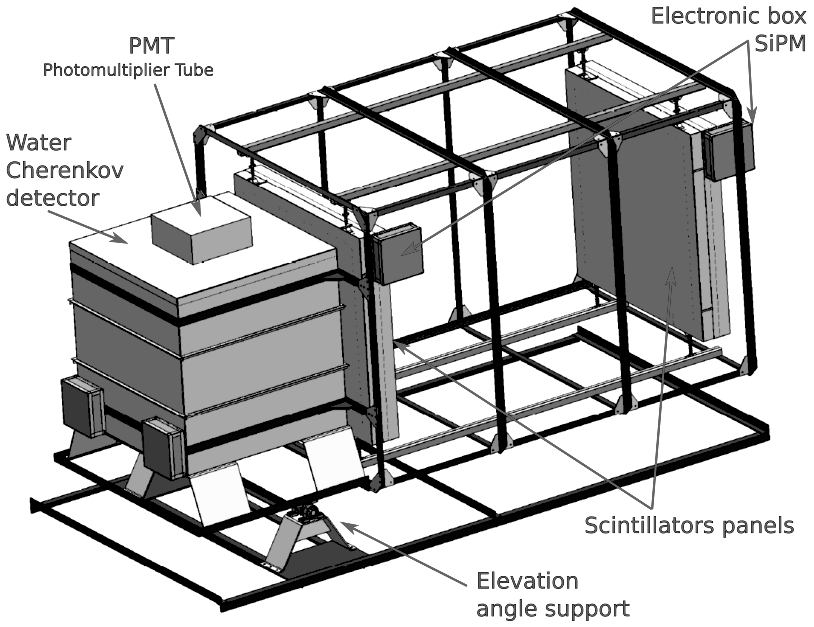
\includegraphics[scale=0.3]{Figures/mute-detector.png}
    \caption{The scketch of the hybrid detector \textsl{MuTe}: a two-panel Scintillator Bars Hodoscope in front and a Water Cerenkov Detector at the back. Each panel of the \textsl{SBH} has $900$ pixels of detection to determine the incoming directions of the particles. The \textsl{WCD} is a metal purified water container of $120$cm side, coated inside by the Tyvek with a \textsl{PMT} on top to detect the Cerenkov photons. It is devised to filter most of the backward \& background noise of muography. The mechanical structure has a variable elevation angle to adjust the telescope according to the object under study.} 
    \label{fig:mute-detector}
\end{figure}



%%%%%%%%%%%%%%%%%%%
%%%% SECTION 2 %%%%
%%%%%%%%%%%%%%%%%%%
\subsection{Hodoscope response to cosmic background radiation}\label{sec:hodoscope-response}
The response of the hodoscope bars refers to the signal produced in the photo-sensor when a minimum ionizing particle (\textsl{MIP}) crosses each scintillation bar. As shown in figure \ref{esquema_centelladora}, charged particles crossing the bars produce scintillation photons, absorbed, re-emitted, and guided to the photo-sensor device by a wavelength shifting (\textsl{WLS}) multi-cladding fiber. 

The bars of \textsl{MuTe} are Dow Styron $663$, made of Polystyrene, doped with $1$\% \textsl{PPO} and $0.03$\% \textsl{POPOP} \cite{PlaBrossRykalin2003}, which place a photon emission peak around the $420$nm wavelength. These bars, coated with $85$\% Polystyrene and $15$\% TiO$_2$ of $0.25$mm thick, have a hole of $\sim 3$mm diameter at its center,  where there is \textsl{WLS} multi-cladding fiber (reference BCF92 of Saint Gobain). The fiber diameter is $1$mm, with a core made of Polymethyl methacrylate, having the first clad of Polyethylene, and the second one of Fluorinated Polyethylene \cite{SaintGobain2017}. A mechanical coupling joins the fiber with a silicon photo-multiplier (\textsl{SiPM} S13360-1350CS of Hamamatsu), with a photo-sensitive surface of $1.3$cm $\times 1.3$cm of $2668$ pixels \cite{Hamamatsu2018}. This device has a spectral detection range from $270$ to $900$nm, with its maximum sensitivity around $450$nm.

\begin{figure}[h!] %Rocal
    \centering
        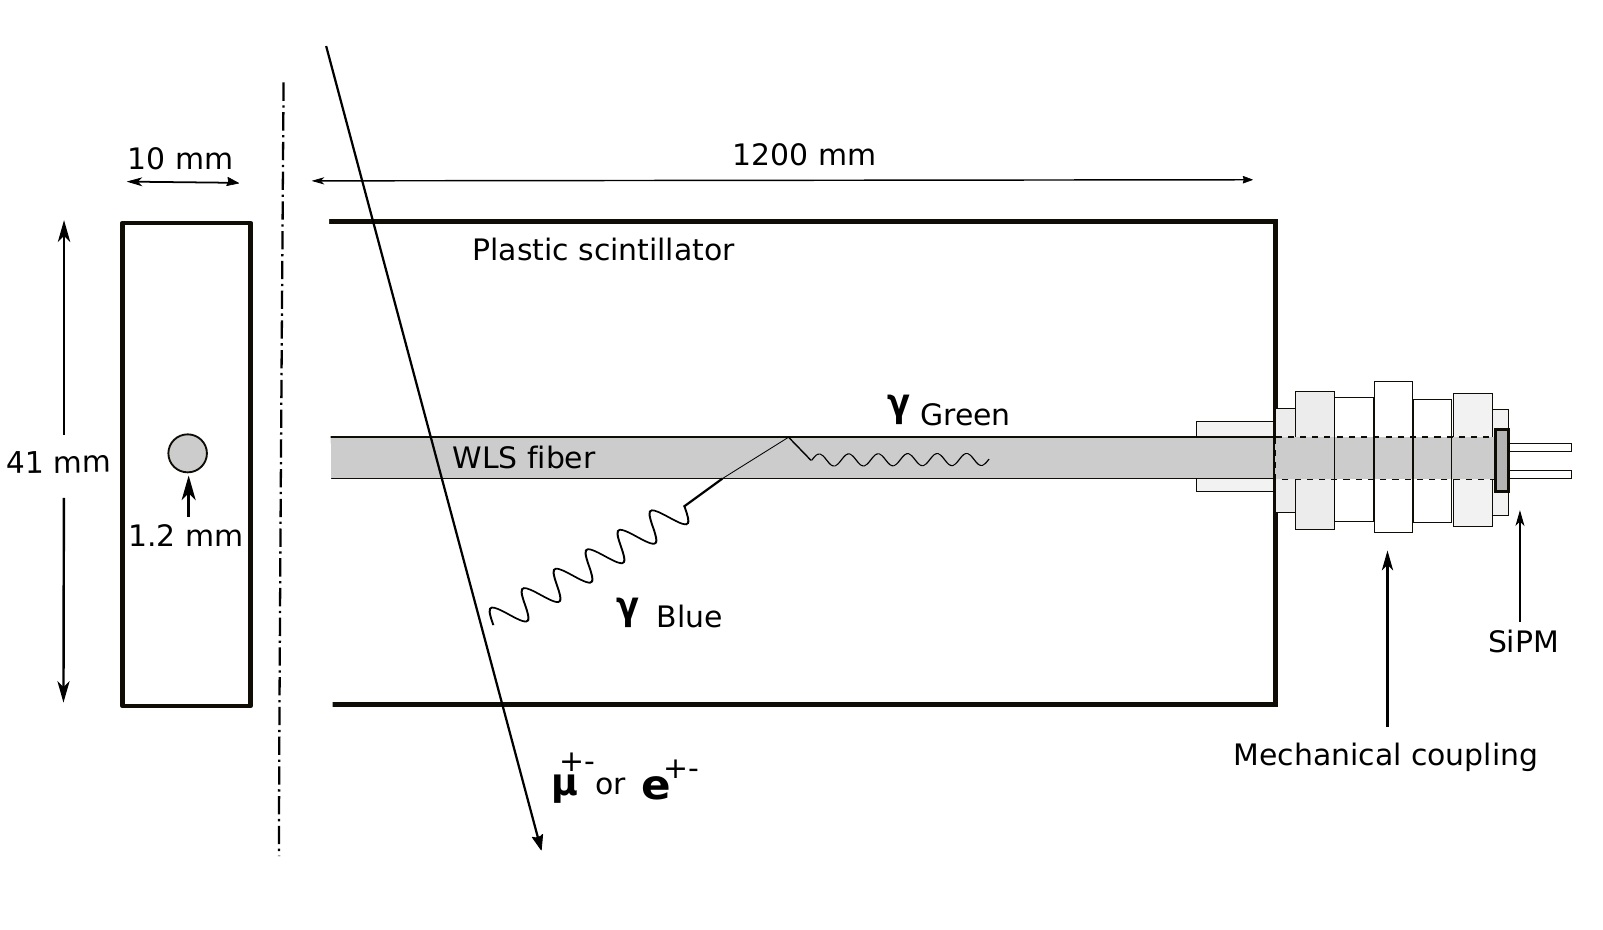
\includegraphics[scale=0.21]{Figures/esquema_barra.jpeg}
   \caption{This picture represent the scintillator bar system, with an embedded \textsl{WLS} fiber used for the experimental study of plastic scintillators coupled to \textsl{SiPM}, what is remarkable, plastics are chosen to change the wavelength. When a charged particle cross the bar it losses part of its energy that generates photons with wavelength around the blue. Those photons are absorbed and re-emited in the fiber as green photons. This fiber guides the photons to the SiPM where they produce a signal depending on their wavelenght (its spectral detection range is $270$ to $900$nm with the maximum sensivity around $450$nm).}\label{esquema_centelladora}
\end{figure}

Next Sections will discuss the \textsl{Geant4} simulation model of the bars, as well as the experimental setup for the analysis of their responses (see section \ref{sec:bar-data}) and estimation of the average response of the hodoscope panels to the passage of \textsl{MIPs} (see section \ref{sec:hodoscope-response-two}). %On the other hand, the first data taken with the \textsl{SBH} in the laboratory are shown in section \ref{sec:hodoscope_data}. 


%%%%%%%%%%%%%%%%%%%%%%%%%%%
%%%%%%% SUBSECTION %%%%%%%%
%%%%%%%%%%%%%%%%%%%%%%%%%%%
\subsubsection{The scintillator bar model} \label{sec:bar-simulation}%Adriana
The scintillator bar \textsl{Geant4} geometric model is a parallelepiped of $4$ cm wide, $2$cm high, $120$cm long and $0.25$mm. We incorporate to this geometry a coating material --made of $15$\% of TiO$_2$ and $85$\% of polystyrene-- with a reflectivity of 1. The scintillating bar is polystyrene, with an index of refraction, $n =1.50$, and a photon absorption length of $5.5$cm. There is a tunnel of $119.5$cm long and $1.8$mm diameter through the main axis of the bar, where we place a multi-cladding \textsl{WLS} fiber. This looseness of $0.5$cm at the end of the tunnel --filled with air to make the model as real as possible-- avoids the escape of photons.

A solid cylinder of poly-methyl methacrylate, with $119.45$cm long and $0.5$mm radius, models the fiber. This configuration leaves a space of $0.05$cm inside the tunnel to locate the \textsl{SiPM}. The first clad of this fiber was made as a cylindrical shell of polyethylene, with an internal radius of 0.5 mm and an external radius of 0.515 mm. The second one is a shell of fluorinated polyethylene with an internal radius of 0.515 mm and an external radius of 0.530 mm. Both coatings have the same fiber length.

A square surface of a side of $1.3$mm, attached to one of the fiber, represents the \textsl{SiPMs}. The simulations allow to set the \textsl{SiPM} photon detection efficiency, which depends on the wavelength ($\lambda$) of the photon hitting the \textsl{SiPM}, where the highest probability of photo-electrons (\textsl{pe}) generation is around $470$nm \cite{Hamamatsu2018}. 

The simulation results of the scintillator bar response to charged particles, of different energy, in figure \ref{fig:mips}. The histogram of the number of photo-electrons generated by 10.000 electrons of $20$MeV, $100$MeV and $500$MeV, have the same profile as those corresponding to the $10000$ muons of $1$GeV, $10$GeV and $100$GeV. Therefore, this detector is not able to distinguish muons from electrons. This is the reason why it is necessary to use the \textsl{WCD} to select the muon events from noise. 

\begin{figure}
    \centering
    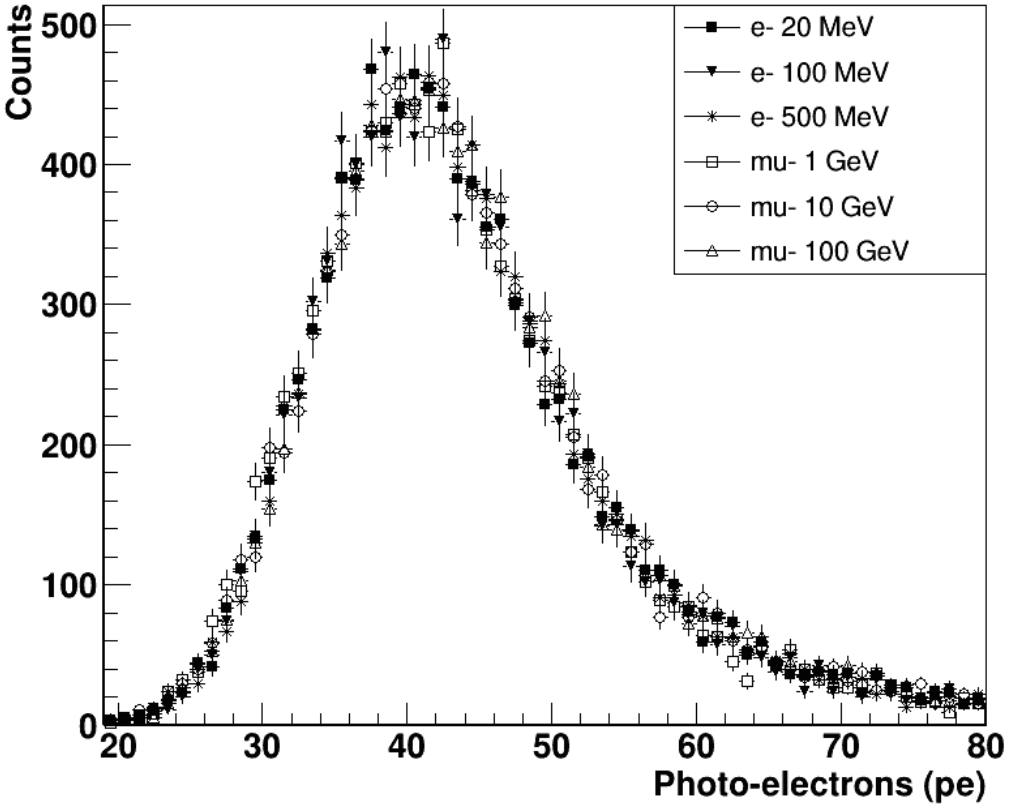
\includegraphics[scale=0.24]{Figures/MIPS.png}
    \caption{Scintillator bar response to \textsl{MIPs} of different energy. As expected, both electrons and muons generate the same histogram profile, since the energy loss of all those particles is $\sim 2$MeV. This result validates the code used and therefore supports the veracity of the simulations of the scintillator bar.
    To obtain those histograms we performed the interaction of 10000 particles (of each energy and type) with the bar. The average number of photo-electrons is around $40$\textsl{pe} for all the particles, i.e. this detector is not able to distinguish muons from noise.}
    \label{fig:mips}
\end{figure}

The mean value of those histograms is around 40 pe. For muons with energy of the order of GeV, the stopping power in the polystyrene is  $\frac{dE}{d\varrho_\mathrm{pol}}\approx 2 \,\text{MeV cm}^2\text{/g}$ \cite{MichaelEtal2008}. Since those particles pass through the bar vertically, the distance traveled is $l_\mathrm{pol}=1$ cm. Hence, $40$\textsl{pe} is equivalent to $2.08$MeV of energy deposited in the bar ($E_\mathrm{d}$), according to equation \ref{energy_deposited}, where $\rho_\mathrm{pol}=1.04$ g/cm$^3$ is the polystyrene density. 

\begin{equation}
\label{energy_deposited}
\begin{split}
    E_\mathrm{d} &= 2 \,\text{MeV cm}^2\text{/g} \times \varrho_\mathrm{pol} \\
    &= 2 \,\text{MeV cm}^2\text{/g} \times l_\mathrm{pol} \times \rho_\mathrm{pol}\\
    &= \text{2.08} \, \text{MeV}.
\end{split}
\end{equation}.

The following simulations were performed with 3 GeV muons, as they are the most likely at the level of the observation point on the Cerro Machín (\textsl{CM}) volcano. That is, from now on the \textsl{MIP} refers to this particle.

%%%%%%%%%%%%%%%%%%%%%%%%%%%
%%%%%%% SUBSUBSECTION %%%%%
%%%%%%%%%%%%%%%%%%%%%%%%%%%
\subsubsection{Attenuation of the photons in the fiber}%Adriana
In order to determine if there is an attenuation in the number of photons that travel through the fiber, a simulation that counts the number of \textsl{pe} generated in the \textsl{SiPM}, when the muon impacts in the normal direction to the bar and at different points, was performed. The initial position of the particle is chosen in such a way that it hits the center of the detection pixels defined for the panels of the hodoscope. For example, if the muon impacts on the center of the first pixel, $P_{1,1}$, its initial position is defined at 2 cm from the \textsl{SiPM}. In this way, the initial position of the muon to hit the midpoint of each pixel is defined as
\begin{equation}
\label{positions}
x_p = (2 + 4p)\mathrm{cm} \,\,\,\,\,\,\,\,\,\, y_p = 1\mathrm{cm}  \,\,\,\,\,\,\,\,\,\, z_p = 2\mathrm{cm},
\end{equation}
with $ y_p $ and $ z_p $ fixed, and $ p = 0,1,2, ..., 29$.

The results of this simulation in figure \ref{atenuacion_barra}, where the fit of the curve is associated with a double exponential function $F(x)$ given by 
\begin{equation}
F(x)= \text{0.468} e^{-0.003(2-x)} + \text{0.531}e^{0.005(2-x)},
\end{equation}
where $x$ represents the impact position of the muon with respect to the \textsl{SiPM}. 

\begin{figure}[h!]
    \centering
        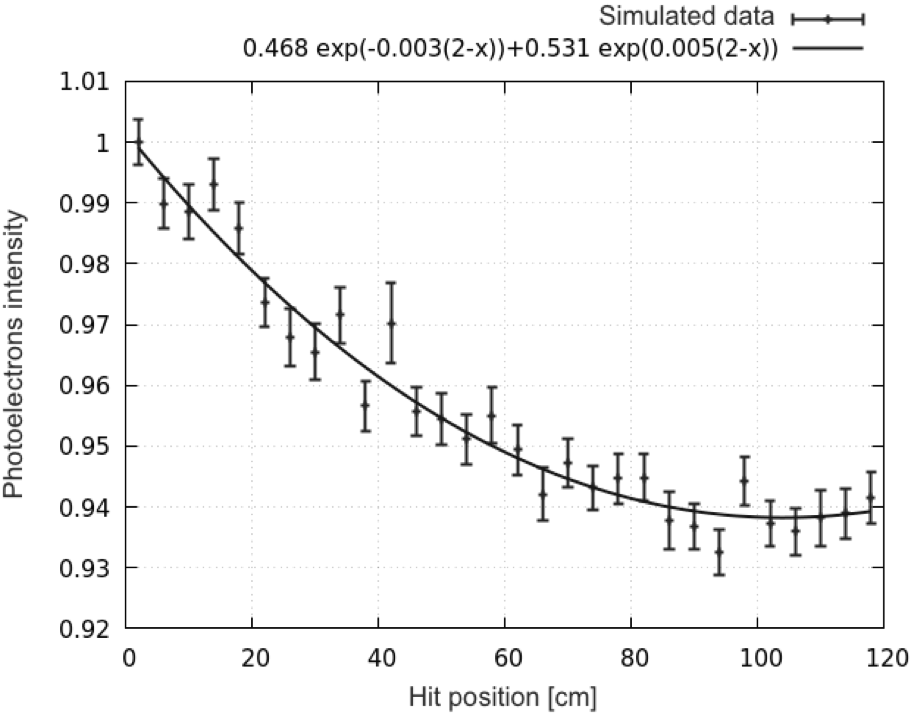
\includegraphics[scale=0.41]{Figures/atenuacion_barra_2.png}
   \caption{Number of photo-electrons with respect to the hit position of the muon in the bar. At $2$cm of the \textsl{SiPM} there are $40$\textsl{pe} on average and at $118$cm there are $37$\textsl{pe}. The difference of \textsl{pe} at the opposite end to the \textsl{SiPM} is approximately $7$\% with respect to the position closest to it. A double exponential function fits the decrease of the simulated data with the hit position $x$. This behavior can be associated with the attenuation of the photons that travel in the fiber.}\label{atenuacion_barra}
\end{figure}

The ends of the scintillator bar and the total number of \textsl{pe} produced in each one presents a slight difference. Having then that at $2$cm of the \textsl{SiPM} an average of $40$\textsl{pe} is produced while at $118$cm $37$\textsl{pe} is produced. From this simulation, the attenuation given is around $7$\%, that is agree with the experimental results given by figure \ref{experimental attenuation}. This difference could be associated with the attenuation of the photons that travel along the fiber.

The \textsl{MIP} detection with scintillator bar generates a number of \textsl{pe} in the \textsl{SiPM} at a time $t$. From the top of the figure \ref{cumulative} it can be noticed that 40\% of the total photo-electrons occurred in the first 10 ns when the muon has entered at 2 cm of the SiPM, while in the bottom of the figure \ref{cumulative} when the muon has entered at 118 cm of the SiPM, only 12 \% of the \textsl{pe} is produced in the same time. In both cases, the total number of \textsl{pe} is reached around $80$ns, that is, the average time necessary to collect the total of \textsl{pe} produced by the passage of a muon, at any point of impact in the bar.

\begin{figure}
    \centering
    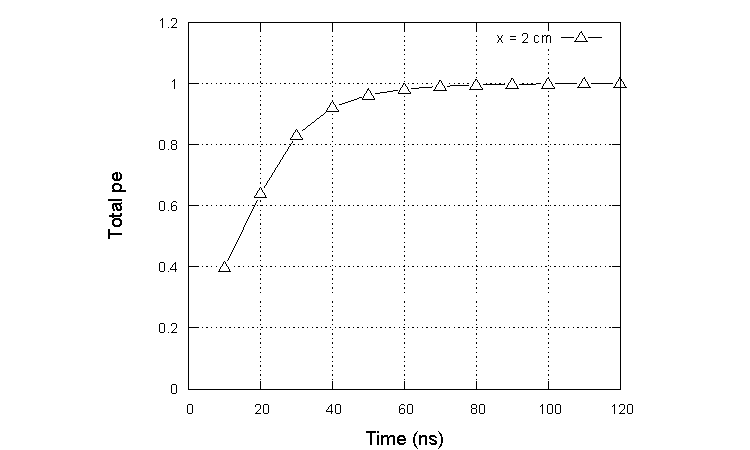
\includegraphics[scale=0.8]{Figures/cumulativo_1.pdf}
    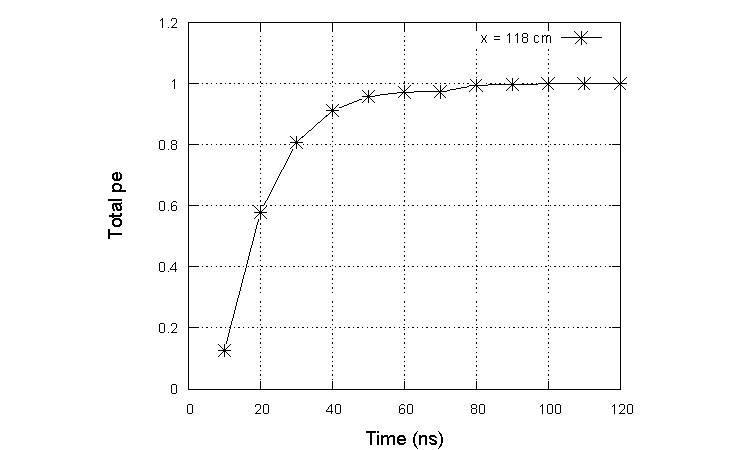
\includegraphics[scale=0.8]{Figures/cumulativo_2.pdf}
    \caption{Cumulative number of photo-electrons produced when a \textsl{MIP} hit the bar at $2$cm from the  \textsl{SiPM} (top) and at $118$cm (bottom). It can be noticed that $40$\% of the Total \textsl{pe} occurred in the first $10$ns when the muon has entered at $2$cm of the \textsl{SiPM}, while, when the muon has entered at 118 cm of the SiPM, only $12$\% of the \textsl{pe} is produced in the same time. In both cases, the total number of \textsl{pe} is reached around $80$ns, that is, the average time necessary to collect the total of \textsl{pe} produced by the passage of a muon, at any point of impact in the bar.}
    \label{cumulative}
\end{figure}

%%%%%%%%%%%%%%%%%%%%%%%%%%%
%%%%%%% SUBSUBSECTION %%%%%
%%%%%%%%%%%%%%%%%%%%%%%%%%%
\subsubsection{ \textsl{SiPM} and fiber coupling}%Adriana
To guarantee an ideal coupling between the \textsl{SiPM} and the fiber, it is necessary to know the number of generated photo-electrons and compare it with a non-ideal coupling. The \textsl{Geant4} model allows estimating these results. Therefore, the ideal coupling is defined as the fiber and the \textsl{SiPM} are side by side without space between them, so all the traveling photons at the edge of the fiber impacts directly in the \textsl{SiPM}. In this case, the passage of the \textsl{MIPs} in the bar was simulated at a distance of $2$\,cm from the \textsl{SiPM} position. As shown above, the obtained average number of photo-electrons, for an ideal coupling, is $40$pe. A non-ideal coupling was generated with a distance of 1.15 mm between the  \textsl{SiPM} and the fiber. The space between them is full of air. In this case, the number of \textsl{pe} is reduced to $8$, representing a loss of 80\% of the signal compared to the ideal case as shown in figure \ref{coupling}.
\begin{figure}
    \centering
    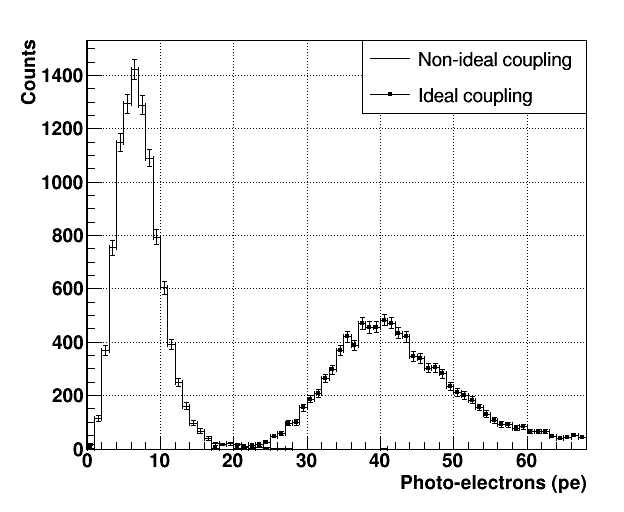
\includegraphics[scale=0.41]{Figures/coupling.png}
    \caption{Histogram of the number of \textsl{pe} resulting from the evaluation of the \textsl{SiPM} and fiber coupling. The squares curve represents the photo-electrons produced in the ideal case (when the \textsl{SiPM} and the fiber are side by side), while the simple line shows the non-ideal case, where the distance between the \textsl{SiPM} and the fiber is $1.15$mm. The average number of \textsl{pe} in the ideal case is around $40$ and in the non-ideal is around $8$\textsl{pe}, i.e. the $80$\% of the signal is lost. This result gives an idea of when a bar-fiber-SiPM system of the real detector is badly coupled, to be replaced or verified.}
    \label{coupling}
\end{figure}


%%%%%%%%%%%%%%%%%%%%%%%%%%%
%%%%%%% SUBSECTION %%%%%%%%
%%%%%%%%%%%%%%%%%%%%%%%%%%%
\subsubsection{Experimental results from the scintillator detector}\label{sec:bar-data}%Rolando
%\textit{(Description of Rolando's methodology and the results: number of photoelectrons per pixel and attenuation) }
The \textsl{MuTe} panels are build of plastic scintillators, these are active detectors  and  work as counters of charged particle. This allows the indirect detection of ionizing radiation. The light that is produced at the passage of charged particles is converted in electrical signals. The last step is the offline analysis. The diagram of the module is represented in figure \ref{esquema_centelladora}. 

To use the fiber and \textsl{SiPM} coupled system, a first study was made to guarantee that the \textsl{SiPM} keeps working in Geiger mode at any temperature. This allows to define a methodology to detect particles with the coupled system. %if there is background noise.
Since the system has an intrinsic noise, it is important to know the detection system and have a strategy of interpretation of the measured data, to have a discriminant. Next section presents the results of the dependence of the breakdown voltage with the temperature.

On the other hand, given that scintillators and \textsl{SiPM} are not $100$\% efficient, there are various parameters to take into account. For example, the material of the bars is opaque to photons with an average length of $4$cm of attenuation. Then, in order to have a detector of $120$cm length, a \textsl{WLS} fiber is placed inside the bar. The fibers guide the photons, but they can present attenuation in spite of being multi-layer, i.e. some photons can escape from the guide and even be reflected in the border. This represents an additional problem when coupling different scintillators and there will be edge effects related to the refractive index of each one.
In addition, to have a larger detection area, we must quantify the attenuation in these fibers and determine, in the case of the MuTe detector, whether the coupling and attenuation will be relevant. To answer these questions, a controlled experiment was performed, to estimate the percentage of attenuation in the system and a counting strategy.

%%%%%%%%%%%%%%%%%%%%%%%%%%%
%%%%%%% SUBSECTION %%%%%%%%
%%%%%%%%%%%%%%%%%%%%%%%%%%%
\subsubsection{Dependence of the breakdown voltage with the temperature}%Rolando

To study the response of each scintillator bar, the stability of the \textsl{SiPM} to temperature changes was first studied. For this purpose, a temperature controlled box was built. This box was regulated by a TEC1-12706 thermoelectric peltier, mounted on an aluminum frame where the mechanical coupling with the \textsl{SiPM} was located. 
This structure was introduced in a thermally insulated box. The control system consist of two sensors: one to vary the temperature and the other one to measure the temperature of the \textsl{SiPM}. To define a target temperature, measurements of the time the system was set up were made. The measurements were taken with the following temperatures: $10^{\circ}$C, $20^{\circ}$C,  $40^{\circ}$C and $50^{\circ}$C. It was concluded that the time required to reach the target temperature was around 600s $\pm$ 50s.

The \textsl{SiPM} power supply was then mounted and the DarkCurrent \cite{Renker2006} was measured in the range of $40$V to $60$V. This was done for $5$ target temperatures, $0^{\circ}$C, $10^{\circ}$C, $20^{\circ}$C, $30^{\circ}$C, $40^{\circ}$C, $50^{\circ}$C for each temperature. There was a curve from which the rupture voltage was calculated, the relationship between the rupture voltage and the temperature in figure \ref{temperature}. From this was determined that for each $10^{\circ}$C the breaking voltage of the \textsl{SiPM} varies 0, 45V.

\begin{figure}[h!] %Rocal
    \centering
        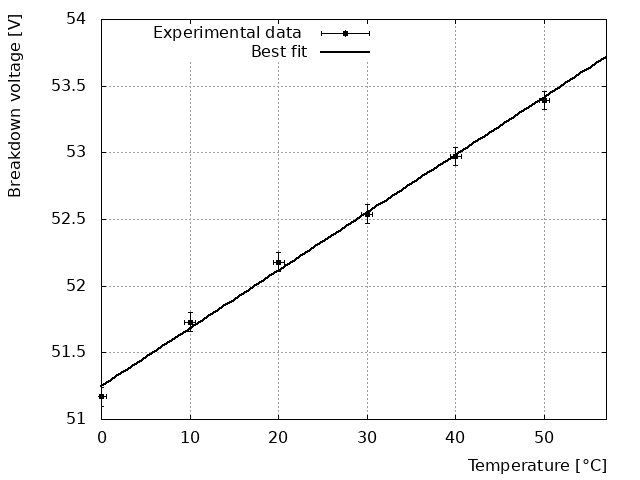
\includegraphics[scale=0.49]{Figures/voltajeRuptura.png}
   \caption{Relationship between temperature and Breakdown Voltage for the  \textsl{SiPM} Hamamatsu S13360-1350CS used in the MuTe telescope.}\label{temperature}
\end{figure}

%%%%%%%%%%%%%%%%%%%%%%%%%%%
%%%%%%% SUBSECTION %%%%%%%%
%%%%%%%%%%%%%%%%%%%%%%%%%%%
\subsubsection{Attenuation measurements of the scintillator bar system}%Rolando

%The light propagating inside the scintillator and the \textsl{WLS} fiber has an inevitable attenuation, some photons escape from the optical guide and others are simply absorbed by the material while being transported to the \textsl{SiPM}.
In order to calculate the attenuation in the scintillator bars, an assembly of scintillators in coincidence was carried out inside the black box. The scintillators were placed on a frame that slid on a rail along the test bar as shown in figure \ref{coincidencia_barras}. These scintillators worked in coincidence in order to generate a trigger signal required to save the pulse on the test bar. Three important positions were chosen: the opposite end of the coupling location, in the middle of the scintillator bar and at the end where the  \textsl{SiPM} was located.

\begin{figure}[h!] %Rocal
    \centering
        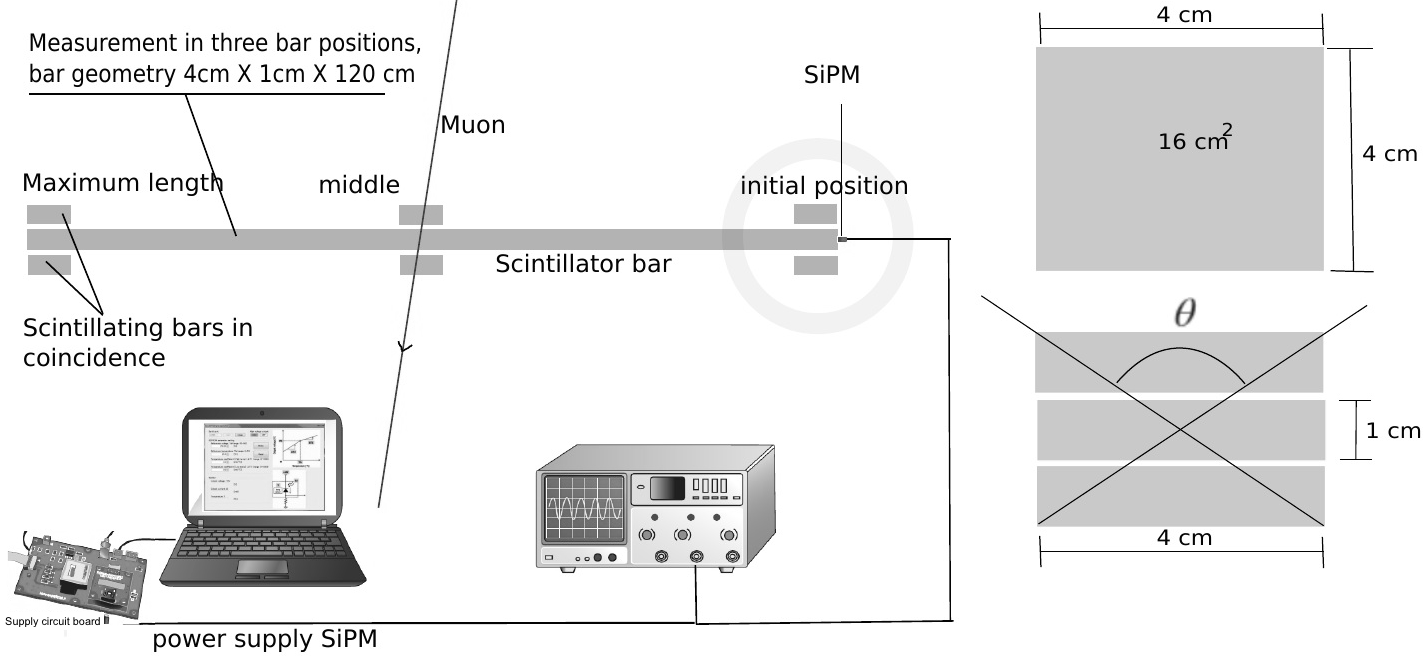
\includegraphics[scale=0.23]{Figures/barras_coincidencia.png}
   \caption{Schematic layout of the experimental set-up.} \label{coincidencia_barras}
\end{figure}

To generate the trigger signal, small scintillators with rectangular cross-section and dimensions ($4$cm $\times$ $4$cm $\times$ $1$cm) were used. They also had \textsl{WLS} fiber and a \textsl{SiPM} in each scintillator. This trigger system was connected to a RedPitaya development card capable of recording pulses with a frequency of 125 Mhz (cite). The system was synchronized to have pulses in coincidence, having three input signals to the card and one output signal that corresponded to each position in the scintillator bar of study.

After performing a calibration with respect to the noise, $10000$ reference pulses were taken in the three positions of interest. In the position opposite to \textsl{SiPM}, the fiber was cut to $45^{\circ}$ to maximize photon leakage and avoid secondary pulses by reflections at the end of the fiber. However, reflections are practically inevitable.

The coinciding system had an angle $\theta$ for this configuration of $106.26^{\circ}$ as shown in the figure \ref{coincidencia_barras}. The frequency of events per minute that was measured experimentally with the aid of an oscilloscope was $10\pm1$ per minute for $16$cm$^2$. With these data was estimate that were detected 0.62 particles$\times$min$\times$cm$^2$. \\



\begin{figure}[h!] %Rocal

    \centering
        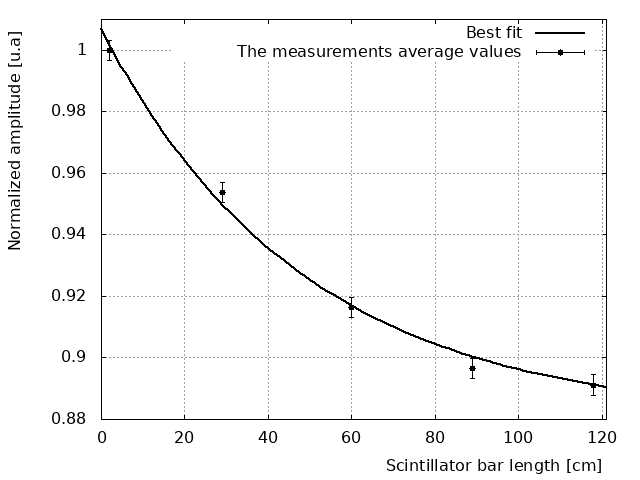
\includegraphics[scale=0.49]{Figures/atenuacion_esperimental.png}
   \caption{Porcentual attenuation from scintillators system.} \label{experimental attenuation}
\end{figure}

---- Explicación media de carga depositada -----  en progreso----


%%%%%%%%%%%%%%%%%%%%%%%%%%%
%%%%%%% SUBSECTION %%%%%%%%
%%%%%%%%%%%%%%%%%%%%%%%%%%%

%%%%%%%%%%%%%%%%%%%%%%%%%%%
%%%%%%% SUBSECTION %%%%%%%%
\subsubsection{Simulated attenuation in the hodoscope}
\label{sec:hodoscope-response-two} %Adriana
To determine the response of each panel of the hodoscope the probability of producing photo-electrons in the \textsl{SiPM} of a horizontal bar and in a vertical bar is taken into account. Those events are independent one from the other, therefore for the front panel the probability in the pixel $P^{F}_{i,j}$ is given by 
\begin{equation}
\label{pe_panel}
P^{F}_{i,j}=P^{F}_{i} \times P^{F}_{j},
\end{equation}
where $P^{F}_{i}$ y $P^{F}_j$ are the probabilities obtained in the horizontal bar $i$ and in the vertical bar $j$, respectively.

From the bar simulation results, the response of a detection panel to \textsl{MIPs} can be obtained. Following the equation \ref{pe_panel}, the probability of photo-electrons produced by \textsl{MIPs}, which have hit each of the pixels of the panel, was obtained and shown in the figure \ref{atenuacion_panel_bw}.

\begin{figure}[h!]
    \centering
        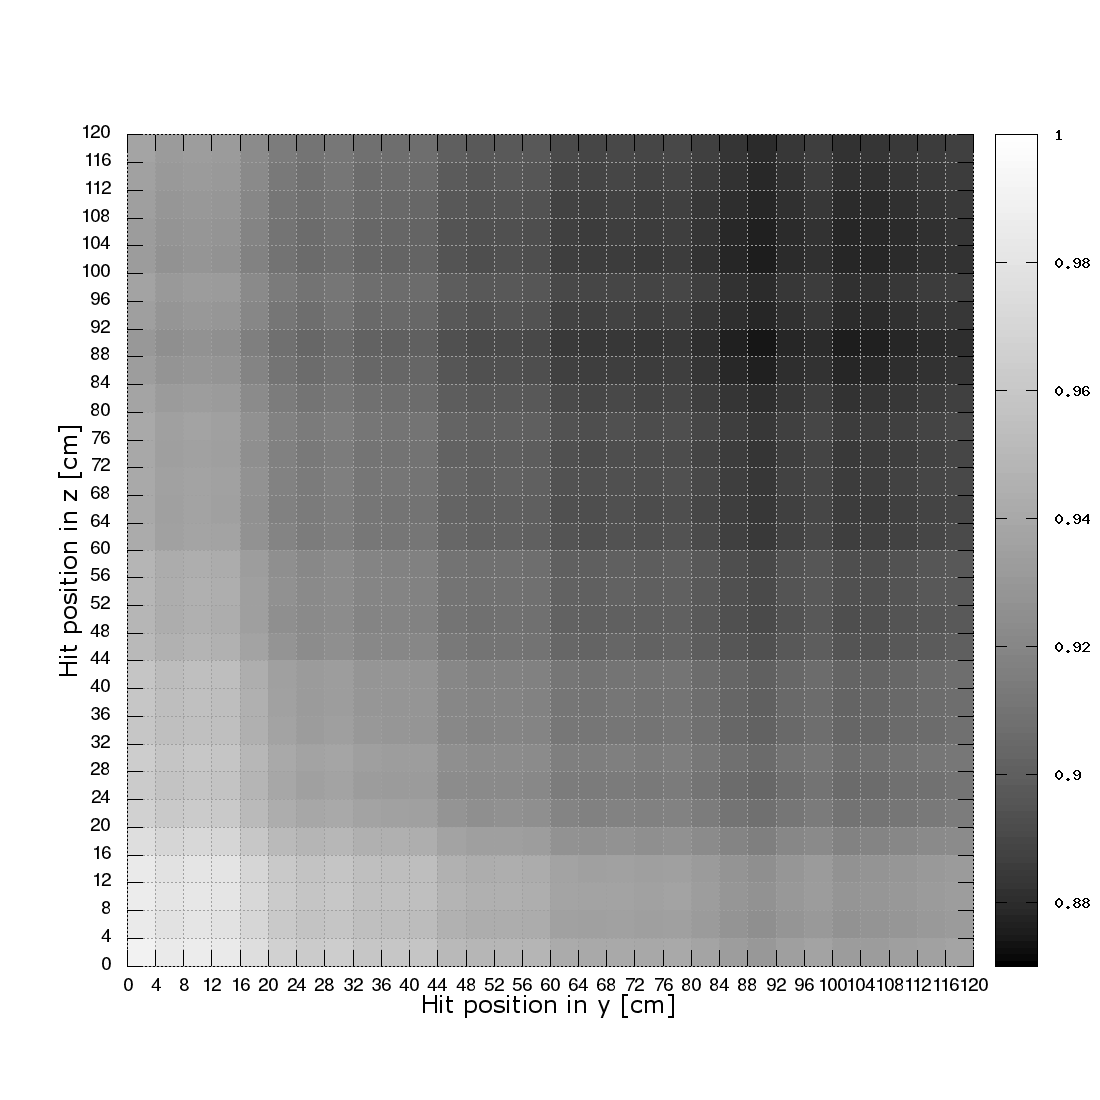
\includegraphics[scale=0.3]{Figures/atenuacion_panel_bw.png}
   \caption[Response of the hodoscope panels]{Production probability of photo-electrons in each of the pixels of a panel of the hodoscope by muons of 3 GeV of energy. Each frame represents a detection pixel and it can be seen that there is a difference between two zones of the panel. In the pixel $P_{11}$, where the \textsl{SiPM} of the horizontal bar and the vertical bar is only 2 cm from the point of impact of the muon, is produced the maximum number of \textsl{pe} while the \textsl{pe} decreases until 12\% for pixels far from the SiPMs. This result is valid both for the front and the rear panel.}\label{atenuacion_panel_bw}
\end{figure}


These results are valid for both the front panel and the rear panel, and it is observed that there is a difference between the zones of the graphic \ref{atenuacion_panel_bw}. This difference around $12$\% is associated to the attenuation of photons in the fiber, that is, the pixels that are closer to the \textsl{SiPM} count more photo-electrons. 


%%%%%%%%%%%%%%%%%%%%%%%%%%%
%%%%%%% SUBSECTION %%%%%%%%
%%%%%%%%%%%%%%%%%%%%%%%%%%%
%\subsubsection{First hodoscope measurements}\label{sec:hodoscope_data} %Jesus

%In order to compare the scintillator panel performance with simulation results we carried out flux measurements. The amplification of the scintillation signals comings from the \textsl{SiPMs} is of 92 times, using an operational amplifier OPA691. On the other hand, discrimination was made with the 64 channels of the ASIC MAROC3A, setting a discrimination threshold by a 10 bits digital-to-analog converter. 

%Many factors cause variations in the bar detection rate. These are the scintillator material impurities, \textsl{WLS} fiber assembling,  \textsl{SiPM} coupling, signal conditioning, and transmission. Taking into account those variables, the hodoscope calibration must start with an equalization stage of the bar response by applying a weighted gain per channel. The equalization is carried out reducing the variability around the mean detection rate, that is, increasing the gain for channels under the mean and decreasing the gain for channels above the mean. The results displays an average detection rate of $8363$ $\pm 96.3$ event/h per bar. 
%Furthermore, a bad optical coupling is exemplified in bar $Y_{26}$ because of its low rate even after equalization.

%\begin{figure}[h]
 %   \centering
  %  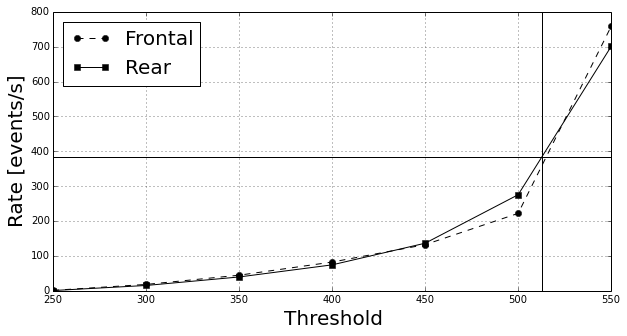
\includegraphics[scale=0.38]{Figures/Panel_cal.png}
   % \caption{Detection rate for the frontal and rear panel ranging discrimination thresholds from 250 UDAC to 550 UDAC. The red cross indicates the discrimination value for a 384 events/s expected rate at 990 m.a.s.l. }
    %\label{PanelRate}
%\end{figure}

%Afterward, the hodoscope was placed inside a laboratory under a 30 cm concrete shielding for performing the calibration using cosmic muons. The threshold value was set taking into account the expected muon rate in an area of 14400 cm$^²$ at  990 m.a.s.l ($\sim$ 1.6 muon/cm$^²$min). Fig. \ref{PanelRate} shows the detection rate for the frontal and rear panel depending of the discrimination threshold value (V$_{th0}$). The  expected rate is about 384 events/s which means a threshold of 510 DAC units.

%Otherwise, the number of photons reaching the  \textsl{SiPM} depends on the interaction point, the higher the distance between the  \textsl{SiPM} and the interaction point, the higher the attenuation in the photon yield. After analyzing 15 hours of data recording with the hodoscope pointing to 0 degrees zenith, it was found that the scintillator panel is less sensitive in average up to 40 $\%$ in the furthest corner from the  \textsl{SiPM} placement as in Fig. \ref{PanelData}.

%\begin{figure}[h]
 %   \centering
  %  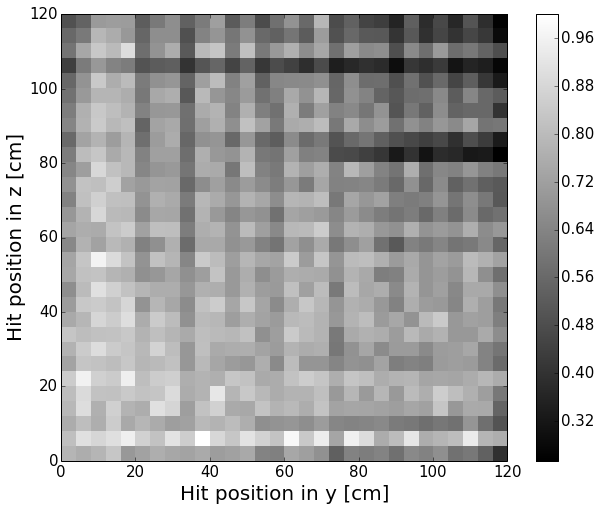
\includegraphics[scale=0.38]{Figures/PanelData.png}
   % \caption{Normalized hit histogram for the frontal panel with 15 hours of data. The locations of the \textsl{SiPMs} are in the bottom-left corner (0,0). In the furthest corner (120cm, 120cm) the detection rate decrease down to 30$\%$. }
    %\label{PanelData}
%\end{figure}

%%%%%%%%%%%%%%%%%%%
%%%% SECTION 4 %%%%
%%%%%%%%%%%%%%%%%%%
\subsection{The water Cerenkov detector response to cosmic background radiation}\label{sec:wcd-response}
The \textsl{WCD} indirectly detects charged particles, counting the Cerenkov photons that originate when the particle travels a certain length in the water. The counter is a photo-multiplier tube, that generates a number of photo-electrons according to its quantum efficiency. This efficiency depends on the wavelength of the photon that reaches it, in this case, the \textsl{PMT} Hamamatsu R5912 of the \textsl{MuTe} has a maximum detection probability value of $25$\% for photons with $\lambda = 400$ nm \cite{Hamamatsu2018}. This \textsl{PMT} is located at the center top of the \textsl{WCD}. As stated above, this detector is a metal purified water container of $120$\,cm side, coated inside by the Tyvek to spread the photons that reach the walls of it, and thus ensure that the maximum number of Cerenkov photons reach the \textsl{PMT}. 

The following sections show the results of the simulation of the response of this detector to charged particles, as well as the first data recorded by the real \textsl{WCD} in the laboratory.


%%%%%%%%%%%%%%%%%%%%%%%%%%%
%%%%%%% SUBSECTION %%%%%%%%
%%%%%%%%%%%%%%%%%%%%%%%%%%%
\subsubsection{The WCD model}\label{sec:wcd-model}
The simulated water container in \textsl{Geant4}, is a cube of length $l_c=1.21$m, made of stainless steel. The water occupies a cube of $ l=1.20$m side with a refractive index $n$, which varies between $1.3435$ and $1.3608$, and a photon absorption length ranging from $0.69$m to $2.90$m according to its energy. In the walls of the water cube the Tyvek is modeled as an optical surface with reflection index $n_{\mathrm{Tyvek}} = 1 $, which diffuses the Cerenkov photons.

For the \textsl{PMT}, the photo-cathode was simulated as an air half-ellipsoid with semiaxes $s_x=10.1$cm, $ s_y = 10.1$cm and $s_z=6.5$cm, located on top of the water cube. The quantum efficiency of this device was introduced into the code, so that the photons that reach the outer surface of the photo-cathode are absorbed or detected, according to the probability of detection given by the R5912-Hamamatsu reference \cite{Hamamatsu2018}. The photons detected, that is, those photons that have enough energy to release an electron from the surface of the photocell by photoelectric effect, are called photo-electrons.
 
It should be noted that the inclusion of the efficiency of the \textsl{PMT} in the code, as a function dependent on $\lambda$, represents an improvement over the simulations of \textsl{WCDs} carried out previously within the research group. An unique efficiency of $25$\% is taken into account in \cite{CalderonAsoreyNunez2015}, for the wavelength range between $330$nm and $570$nm. Therefore, the new code offers more precise results of the pulses produced by the passage of particles in water. 
 
%%%%%%%%%%%%%%%%%%%%%%%%%%%
%%%%%%% SUBSECTION %%%%%%%%
 \subsubsection{Estimation of the Vertical Equivalent Muon unit}
 To measure the deposited energy by the incident particles, an absolute calibration of the detector is needed. The Vertical Equivalent Muon (\textsl{VEM}) is generally adopted as the measurement unit of calibration \cite{EtchegoyenEtal2005}. This is defined as the average charge collected in the \textsl{PMT} when a high-energy muon crosses the entire detector vertically. In the calibration of the \textsl{WCD} these muons can be easily identified by installing plastic scintillators above and below the detector, centered on their axis \cite{EtchegoyenEtal2005}, so the muon can be detected before and after leaving the \textsl{WCD}.
 
It is not necessary to implement this method in the detector simulation, due to the \textsl{Geant4} code allows to inject muons with a chosen energy and a initial direction. In this case, $100000$ muons were injected with $3$GeV of initial energy, in direction $-\hat{z}$ towards the water, and the initial position given by the point $ P=(80, 80, 121)$ cm, over the \textsl{WCD}. 

As a result, the average number of Cherenkov photons, $N$, produced in the water by those incident particles that have traveled a distance $l$ in water was obtained. The portion of $N$ that reaches the external surface of the photo-cathode is named as $N_{\mathrm{PMT}}$. Finally, the $ N_{\mathrm{PMT}}$ produces a number of photo-electrons, $N_{\mathrm{pe}}$, depending on its wavelength. From this, the \textsl{WCD} efficiency to detect muons was estimated, i.e. a \textsl{VEM} of $3$GeV generates around $46857$ Cherenkov photons in $120$cm of water crossed, only $1617$ of those photons reach the external surface of the photo-cathode and, from its quantum efficiency, around $203$ \textsl{pe} are produced in average. Thus, the system has a muon detection efficiency of $0.4$\%, that is,
\begin{equation}
\eta_{\mathrm{WCD}}=\frac{N_{\mathrm{FE}}}{N} 100\%=\frac{203}{46857}100\%=0\textnormal{.}4\%
\end{equation}


Since the unit of calibration \textsl{VEM} is independent of the site of detection, the simulated value ($\sim 203$ pe) is compared with the value obtained from the first data of the \textsl{WCD} located in the laboratory, that is around $\sim 167.5$pe as shown figure \ref{WCDpe}. 

In order to compare the \textsl{WCD} response to muons and electrons of typical energy at the \textsl{CM} volcano, we compute the same simulations for $100000$ electrons of $20$MeV at the same initial direction and point $P$. These particle are defined as Vertical Electrons (\textsl{VE}) and the histogram of the number of photo-electrons produced in the figure \ref{vem_ve} with the \textsl{VEM} histogram. The mean value of the \textsl{VE} is smaller than the \textsl{VEM}, around $17$\textsl{pe} that represents a $8$\% of it.

Here is also obtained the characteristic pulse for \textsl{VEM} and \textsl{VE} as the number of \textsl{pe} vs time, shown in the figure \ref{pulse_vem_ve}. From those histogram fits we can obtain the attenuation time $\tau$ and lenght $l_a$, of the signal. 

A summarize of the results and a comparison between both particles is shown in the table \ref{t:comparacion}.

\begin{figure}
    \centering
    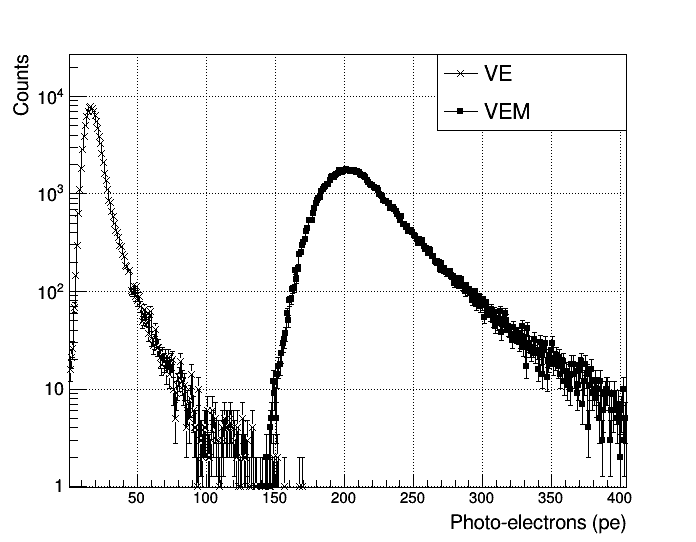
\includegraphics[scale=0.38]{Figures/vem_ve.png}
    \caption{Histogram of the number of photo-electrons produced due the detection of vertical muons (squares) and vertical electrons (crosses) with the \textsl{WCD}. From the squares curve, the mean value for the unit of calibration, \textsl{VEM}, is around $203.2$\textsl{pe}. In comparison, the mean number produced by the \textsl{VE} is $16.7$\textsl{pe}, that is the $8$\% of the \textsl{VE}. This results shows that the \textsl{WCD} }
    \label{vem_ve}
\end{figure}

\begin{figure}
    \centering
    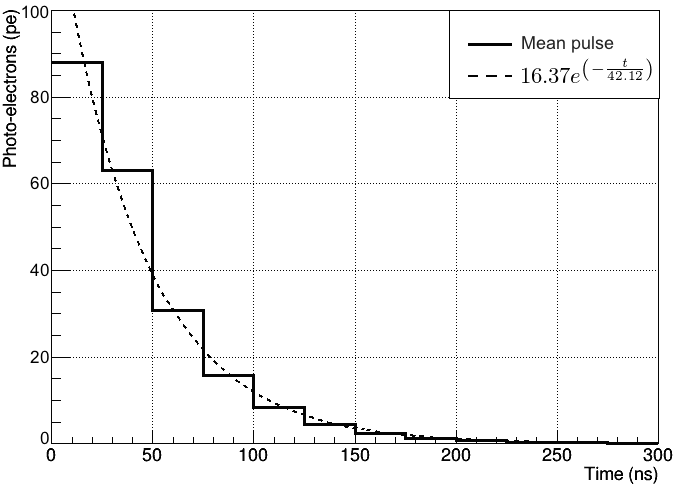
\includegraphics[scale=0.35]{Figures/pulse_vem.png}
    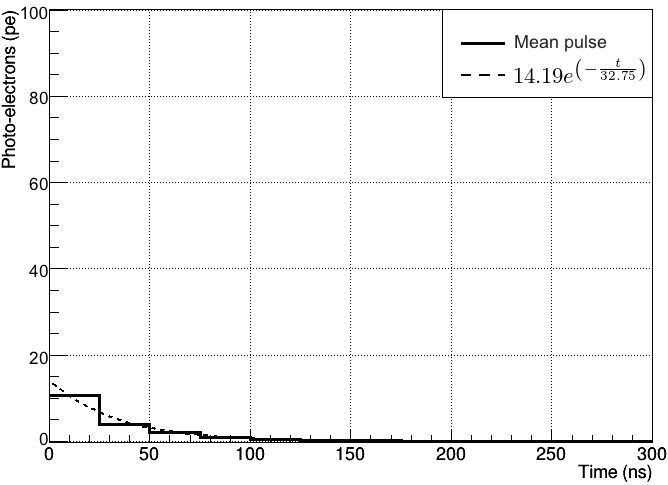
\includegraphics[scale=0.35]{Figures/pulse_ve.png}
    \caption{Mean pulse corresponding to the \textsl{VEM} (top) and the \textsl{VE} (bottom) response. The dashed lines represent the best exponential fit of the pulses where the attenuation time $\tau$ is around $42.12$ns for the \textsl{VEM} and $32.75$ns for the \textsl{VE}.}
    \label{pulse_vem_ve}
\end{figure}

\begin{table}[h!]
\label{t:comparacion}
\centering
\caption{Summary of the physical magnitudes obtained for the \textsl{VEM} and the \textsl{VE}: Length traveled in water ($l$), Number of Cherenkov Photons produced ($N$), Number of Photons that reach the \textsl{PMT} ($N_{\mathrm{PMT}}$), Number of Photoelectrons ($N_{\mathrm{FE}}$), Time of attenuation of the pulse ($\tau $) and Length of attenuation ($l_a$).}

\begin{tabular}{l|c|c|}
\cline{2-3}
                                                     & \textbf{$\mu^-$ (3 GeV) }& \textbf{$e^-$ (20 MeV)} \\ \hline
\multicolumn{1}{|l|}{\textbf{$l$}}   &          (120 $\pm$ 1) cm      &    (10 $\pm$ 1) cm        \\ \hline
\multicolumn{1}{|l|}{\textbf{$N$}}    &         46857 $\pm$ 13 $ $   &      3538 $\pm$ 1 $ $      \\ \hline
\multicolumn{1}{|l|}{$N_{\mathrm{PMT}}$}       &          1617 $\pm$ 1     &     132.1 $\pm$ 0.1      \\ \hline
\multicolumn{1}{|l|}{$N_{\mathrm{pe}}$}       &          203.2 $\pm$ 0.2      &     16.729 $\pm$ 0.003       \\ \hline
\multicolumn{1}{|l|}{$\tau$} &          (42.12 $\pm$ 0.01) ns      &      (32.75 $\pm$ 0.03) ns      \\ \hline
\multicolumn{1}{|l|}{$l_a$} &          (7.332 $\pm$ 0.001) m      &      (9.430 $\pm$ 0.002) m      \\ \hline
\end{tabular}
\end{table}

%%%%%%%%%%%%%%%%%%%%%%%%%%%
%%%%%%% SUBSECTION %%%%%%%%
%%%%%%%%%%%%%%%%%%%%%%%%%%%
\subsubsection{WCD response to the cosmic background radiation}%Adriana
The estimation of the \textsl{WCD} response to the cosmic background radiation flux ($\Xi$), at the CM volcano level, was performed with the \textsl{LAGO} \textsl{ARTI} framework \cite{SarmientoEtal2019}. This toolkit employs a \textsl{Geant4} code to estimate the number of Cerenkov photons detected by the \textsl{PMT}, produced due the interaction of the particles with the water of the \textsl{WCD}. The quantum efficiency of the \textsl{MuTe} \textsl{PMT}, R5912-Hamamatsu, was taken into account to perform this simulation. The \textsl{ARTI} framework uses as input the energy and the momentum of the particles from $\Xi$. This flux is obtained using the \textsl{CORSIKA} code and a geomagnetic correction is applied with the \textsl{MAGCOS} code. To obtain the histogram of the number of photo-electrons, the flux $\Xi$, given by
\begin{equation}
\Xi = \frac{N_{\mathrm{Sec}}}{1\,\mathrm{h}\, 1\,\mathrm{m}^2}, 
\end{equation}
is redistributed in a circular area $A$ located at 1 cm of the top of the \textsl{WCD}. The larger the area the larger the number of particles coming in almost all the zenith angles. In order to get the response of particles coming from $0\leq \theta \leq 80^{\circ}$ we set $A=480$m$^2$ in the \textsl{ARTI} framework. Then the flux is re-written as

\begin{equation}
\Xi_{CM} = \frac{N_{\mathrm{Sec}}}{1\,\mathrm{h}\, 1\,\mathrm{m}^2}, 
\end{equation}
where the number of secondaries at CM level (level m a.s.l.) is $N_{\mathrm{Sec}}=$.

The histogram of the number of photo-electrons produced in the \textsl{WCD} due to the flux $\Xi_{CM}$ is shown in the figure \ref{fig:flux}. The different curves are the contribution of the particles components to the total response (empty circles). It can be noted that this curve has two main peaks, the first one with a contribution of the electromagnetic component and the second one with the muonic component.

\begin{figure}
    \centering
    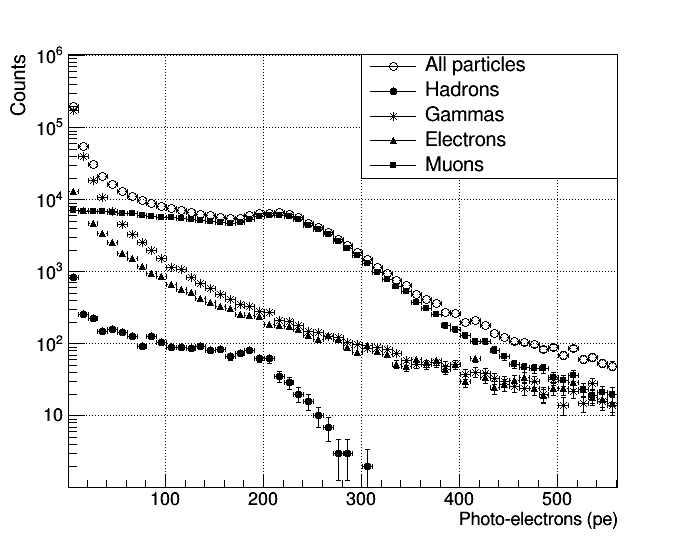
\includegraphics[scale=0.4]{Figures/flux.png}
    \caption{Histogram of the number of photo-electrons produced by all the particles, hadrons, gammas, electrons and muons detected in the \textsl{WCD}.}
    \label{fig:flux}
\end{figure}

%%%%%%%%%%%%%%%%%%%%%%%%%%%
%%%%%%% SUBSECTION %%%%%%%%
%%%%%%%%%%%%%%%%%%%%%%%%%%%
\subsubsection{First WCD measurements}\label{sec:wcd-data}%Jesus

The \textsl{WCD} acquisition system records two signals from the \textsl{PMT}, anode and last dynode. The dynode pulses are amplified 20 times for increasing the measuring range. These two channels are digitized by a 10 bits analog-to-digital converter.

The digitized electric charge $Q_{ADC}$ recorded by the \textsl{WCD} electronics for a charged particle is defined as follows,

\begin{equation}
\label{n_FE}
Q_{ADC} =  \frac{1}{RG_{a}}\sum_{i=0}^{N-1} V_{ADC} \Delta_T
\end{equation}

where $V_{ADC}$ is the digitized voltage, $\Delta_T$ is the time sampling step, $G_a$ is the amplification factor of the electronics front-end, $R$ is the sensitive resistance and $N$ es the number of samples. Then the number of detected \textsl{pe} is,
\begin{equation}
\label{n_FE}
N_{pe} = \frac{Q_{ADC}}{eG_{PMT}}
\end{equation}

where $G_{PMT}$ is the \textsl{PMT} gain and $e$ is the electron charge.

In this case, the \textsl{PMT} was biased with 1kV reaching a $G_{PMT}\sim$0.3$\times10^6$. The conditioning electronics has an amplification factor $G_a = 20$ and $R = 50 \Omega$. The signal is digitized with a sampling frequency of $40$MHz ($\Delta_T$ = 25ns) and stored in a vector of $N$ = 12.  

Fig. \ref{WCDpe} shows the \textsl{pe} histogram for one hour of data for a discrimination threshold of $110$mV. The histogram has two prominent humps, the electromagnetic (electrons, positrons and gammas) hump at $\sim 70$\textsl{pe} and the muonic hump at $\sim 167.5$pe.


\begin{figure}
    \centering
    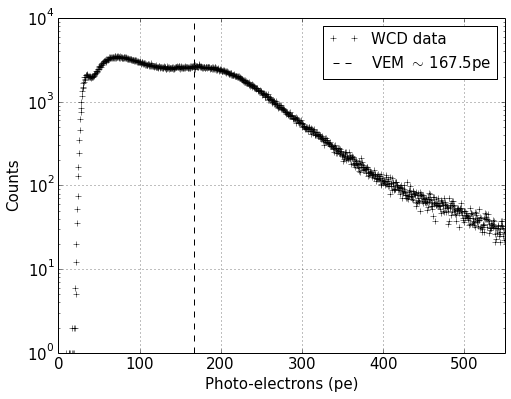
\includegraphics[scale=0.45]{Figures/WCDpedata.png}
    \caption{Photo-electron histogram for one hour of data recorded by the \textsl{WCD}. }
    \label{WCDpe}
\end{figure}



%%%%%%%%%%%%%%%%%%%
%%%% SECTION 6 %%%%
%%%%%%%%%%%%%%%%%%%
\section{Conclusions}\label{sec:conclusions}%Todos

From the \textsl{Geant4} model of the scintillator detector, it was obtained that the number of \textsl{pe} decreases around $7$\% with respect to those produced at the end near of the \textsl{SiPM}. This reduction occurs due to the attenuation of the photons that travel in the fiber, since, the more distance they travel within it, the more energy they lose and are absorbed into the material before reaching the \textsl{SiPM}. This result is in agreement with that obtained with the experimental setup, that is, around $11$\% attenuation. This attenuation seems to be insignificant in the bar, but it is more noticeable in the panels of the hodoscope, since, the difference between the corner of the nearest panel and the one farthest from the \textsl{SiPM}, is around $12$\%.

Regarding to the \textsl{WCD} response, the value of the \textsl{VEM} obtained with the simulations and that obtained in the laboratory, are in the same order of magnitude, but present a percentage difference of $18$\% with respect to the modeled value. This difference can be related by the various components of the electronics, where part of the signal can be lost.

From the results obtained, a muon detection trigger for the \textsl{MuTe} is proposed in terms of the energy deposited in each of its components. That is, the muon must deposit around $2.08$MeV in two scintillator bars on the front panel, then the same energy in two bars on the rear panel of the hodoscope, to finally discriminate the signal from the noise in the \textsl{WCD}. Then, the muon must deposit around 240 MeV of energy in the \textsl{WCD} to be counted as an event.

%Comparación de la atenuación en la barra obtenida por simulación y experimentalmente.

%Atenuación en el panel, no se puede comparar porque la atenuación "teórica" se hizo sacando la integral bajo la curva de cada pulso para obtener el número de fotoelectrones, mientras que la experimental se hizo comparando la atenuación de los picos 
%Comparación del VEM te´rico y experimental: están en el mismo orden de magnitud pero hay una diferencia porcentual del 18% respecto al valor teórico
%decir que tanto simulaciones como resultados fueron obtenidos en bucaramanga, con el "mismo flujo" de partículas.
%Description of the proposed trigger for the detection of muons from the results obtained from the simulation


\bibliography{RefMuTeSimul}


\end{document}